\documentclass[a4paper, 11pt]{article}

\usepackage[utf8]{inputenc}
\usepackage[T1]{fontenc}
\usepackage[francais]{babel} 
\usepackage{amsmath} % pour les formules de maths
\usepackage{amssymb} % pour des symboles
\usepackage{mathrsfs} % pour avoir acces a des jolies lettres calligrafiées.:)
\usepackage{listings} % pour le code source
\usepackage{color} % pour les couleurs
\usepackage{graphicx} % pour les graphiques (images)
\usepackage{fancyhdr} % pour utiliser le pagestyle fancy
\usepackage[headheight=10pt]{geometry} % pour les marges
\usepackage[T1,hyphens]{url}
\usepackage[colorlinks,urlcolor=blue, linkcolor=blue]{hyperref}
\usepackage{float}
\usepackage[perpage]{footmisc}

\geometry{hmargin=3cm}

\title{Projet de Master}
\author{Romain Mencattini}
\date{\today}

\pagestyle{fancy} % pour avoir des entetes et des pieds de page
\renewcommand\headrulewidth{0.6pt}
\fancyhead[L]{Romain Mencattini} % haut de page gauche
\fancyhead[R]{Université de Genève \today} % haut de page droite

\begin{document}
\maketitle
\newpage
\tableofcontents
\newpage

%%%%%%%%%%%%%%%%%%%%%%%%%%%%%%%%%%%%%%%%%%%%%%%%%%%%%%%%%%%%%%%%%%%%%%%%%%
% début de l'état de l'art %%%%%%%%%%%%%%%%%%%%%%%%%%%%%%%%%%%%%%%%%%%%%%%
%%%%%%%%%%%%%%%%%%%%%%%%%%%%%%%%%%%%%%%%%%%%%%%%%%%%%%%%%%%%%%%%%%%%%%%%%%
\section{État de l'art}
\subsection{Introduction}
\paragraph{}
Avant la démocratisation de l'informatique et de son utilisation, toutes les opérations financières étaient réalisées par des humains. Ce système pouvait avoir des inconvénients:
\begin{itemize}
\item L'émotionnel pouvait influer les transactions. En effet, ces dernières étant effectuées par des humains, il y avait une risque non négligeable que l'état de la personne agisse sur sa décision.
\item Un problème sous-jacent était de maintenir une discipline de \textit{trading}. Afin de minimiser les pertes et de maximiser les gains, il fallait se tenir à ce plan afin de ne pas ce laisser influencer par des paramètres extérieurs. Cela pouvait être très difficile.
\item Le \textit{backtesting}\footnote{Backtesting is the process of testing a trading strategy on relevant historical data to ensure its viability before the trader risks any actual capital. [\ref{backtesting investopedia}]} était impossible. Tester la qualification ainsi que la qualité de \textit{trading} d'une personne était compliquée. De même pour un \textit{trading plan}.
\end{itemize}

\paragraph{}
Ces éléments ont, en partie, favorisé l'émergence et l'utilisation d'algorithmes dans la finance. En 2014 aux USA, 84\% des transactions étaient accomplies par des algorithmes [\ref{real investors}]. Ce qui représente environ 100000 réalisations, ou \textit{ticks}, par secondes [\ref{real investors}].
De part l'utilisation intensive de cet outil informatique, le monde de la finance a suivi l'évolution de ce domaine. Afin de perfectionner leurs algorithmes.
On retrouve donc des méthodes d'optimisations poussées ainsi que les récentes découvertes de \textit{data mining} et de \textit{machine learning}, abrégé \textit{ML}. Des propositions de plus en poussées dans les deux domaines voient le jour. L'algorithme qui sera au coeur de ce projet en fait partie. Il s'agit d'un réseau de neurones avec plusieurs couches prenant en compte des paramètres particuliers à la finance.

\paragraph{}Afin d'approcher aux mieux ces notions, nous allons discuter des éléments nécessaires à la compréhension.
Nous allons en premier lieu introduire le domaine financier ainsi que ces outils. Puis nous parlerons de plusieurs méthodes de \textit{ML}.
Voici celles vont être développées dans cet état de l'art:
\begin{itemize}
\item Les réseaux de neurones.
\item Les arbres de décision.
\item Les algorithmes \textit{SVM} [\ref{wikipedia svm}].
\item \textit{Logistic Regression}.
\item \textit{Naive Bayes}.
\item Descente du Gradient [\ref{wikipedia descente du gradient}] ainsi que sa version dite stochastique [\ref{descente du gradient stochastique}].
\end{itemize}

Finalement, nous lierons les deux domaines en montrant comment adapter les modèles mathématiques de \textit{ML} pour les utiliser comme techniques de \textit{trading}.


\subsection{Finance}

\subsubsection{\textit{FOREX}}

\paragraph{}Afin de comprendre le fonctionnement du \textit{FOREX}, il est important de mentionner certaines décisions historiques. Ces dernières ont façonné le marché des devises actuel.

\paragraph{}
Jusqu'à la première guerre mondiale, le système en vigueur se base sur l'or, que l'on nomme l'étalon-or\footnote{Source: [\ref{étalon-or à étalon-dollar}].}. S'en suit une période d'instabilité notamment dûe aux pertes occasionnées par la guerre, un après-guerre compliqué, la crise boursière de 1929 et la seconde guerre mondiale.

C'est au sortir de cette dernière, que la nécessité de "\textit{mettre en place une organisation monétaire mondiale et de favoriser la reconstruction et le développement économique des pays touchés par la guerre}" [\ref{wikipedia bretten woods}], est apparue. Le but était également "\textit{d’aplanir les conflits économiques, reconnaissant par là les problèmes engendrés par les disparités économiques}" [\ref{étalon-or à étalon-dollar}].

Plusieurs propositions furent proposées, mais ce fût celle de Harry Dexter White qu'on mit en place. Cette dernière prévoyait entre autre:
\begin{itemize}
\item le choix du Dollar américain comme étalon, ce dernier étant rattaché à l'or\footnote{Suspension l'équivalence or pour le dollar américain en août 1971 puis abandon définitif en mars 1973 [\ref{wikipedia bretten woods}].}.
\item Création de la Banque internationale pour la reconstruction et le développement (BIRD) qui deviendra la banque mondiale.
\item Le Fond monétaire international (FMI).
\item Création de l'Organisation mondial du commerce\footnote{Ne verra le jour qu'en 1995 faute d'accord [\ref{wikipedia bretten woods}].}.
\end{itemize}

On remarque que ces institutions sont toujours en activité, cela démontre l'importance de ces accords pour comprendre le système financier. Cela est également vrai pour le marché des taux de changes, où le USD est toujours utilisé entre deux échanges.
Il n'est en effet pas possible de faire CHF/EUR\footnote{Franc Suisse - Euro}. Le passage par le USD entre les deux est obligatoire; nous aurons donc CHF/USD\footnote{Franc Suisse - Dollar Américain} puis USD/EUR\footnote{Dollar Américain - Euro}

\paragraph{}
Le marché \textit{FOREX} porte sur les devises. La valeur d'une devise ne peut être exprimée qu'en fonction d'une autre. Par exemple 1 franc suisse vaut 1.05 euro.\footnote{Taux fictif utilisé pour l'exemple.}
La transaction porte donc sur deux monnaies comme CHF/EUR. On va vendre des francs suisses pour acheter euros ou l'inverse.
Le nom du marché vient d'ailleurs de ces échanges. On échange une monnaie contre une autre, c'est un \textit{FOreign EXchange}, ou \textit{FOREX}.

Il y a deux variations de la monnaie possibles:
\begin{itemize}
\item La monnaie peut subir une dépréciation.
\item La monnaie peut subir une appréciation.
\end{itemize}
Lorsque le prix d'une monnaie augmente par rapport à une monnaie étrangère augmente, on parle d'appréciation. Ainsi dans le cas contraire, on parlera d'une dépréciation.

La mondialisation a facilité ce marché. En effet, toutes les devises sont accessibles depuis n'importe où. Il devient donc possible d'avoir des marchés avec des devises plus exotiques.

\paragraph{}
Les principaux acteurs financiers sont [\ref{marche des changes}]:
\begin{itemize}
\item Les banques commerciales. Elles peuvent pratiquer des interventions directes car elles gèrent des dépôts et veulent opérer des transactions sur ces derniers. Il est également possible de réaliser le rôle d'intermédiaire financier.
\item Les entreprises. Ces dernières vont pratique des transactions directes, si elles disposent d'un accès aux marchés sinon via des banques.
\item Les institutions financières non-bancaires. On peut citer les fonds de pensions, les sociétés d'assurances ou les \textit{hedge funds}. Ce sont surtout dans un but de spéculation, d'arbitrage ou de couverture de risque qu'elles interviennent.
\item Les banques centrale. Il peut y avoir des interventions directes, dans le but de modifier l'appréciation de la monnaie.
\item Les ménages. Surtout dans une optique de voyage, d'achat ou de spéculation.
\end{itemize}

\paragraph{}
Henry Bourguinat a énoncé "\textit{la règle des trois unités}" qui correspondent aux unités de temps, de lieu et d'opérations et d'acteurs.
Le \textit{FOREX} répond à ces trois unités [\ref{site fr forex}]:
\begin{itemize}
\item Ce marché fonctionne 24h/24 et les transactions s'effectuent presque en continue.
\item Il fonctionne à l'échelle mondiale tout en étant décentralisé. De part l'évolution des technologies, l'information circule aisément malgré son statut.
\item L'uniformité des procédés ainsi que des produits est présente. Les acteurs malgré nationalité sont de même nature.
\end{itemize}

\paragraph{}
Il existe principalement deux horizon temporels: le \textit{spot} et le {forward}.

Le premier est également appelé "Le marché au comptant". Lorsque deux acteurs se mettent d'accord sur une transaction, cette dernière se réalise immédiatement\footnote{Valable en théorie, dans la réalité cela peut prendre du temps [\ref{marche des changes}]}.

Le second peut être nommé "Le marché à terme". L'accord est passé à un temps $T$ mais la transaction effective ne se réalise que dans le futur. Ce futur, ou maturité, peut être de plusieurs dizaines de jours, voir des années, soit $T + X$.

Il y a opérations réalisable sur le marché à terme.:
\begin{itemize}
\item Les \textit{swaps}. Ils consistent vendre une monnaie au comptant puis à la racheter à terme\footnote{Soit à $T+X$}.
\item Les \textit{futures/forwards}. La différence entre ces deux tient surtout à leur standardisation et leur mise en place. Cependant le principe reste le même: on réalise une opération (d'achat ou de vente) qui ne s'effectuera qu'à maturité.
\item Les \textit{options}. Cela représente un contract vendu par un parti (\textit{the option writer}) à un autre parti (\textit{the option holder}). Ce contrat offre le droit, et non l'obligation contrairement aux \textit{futures/forwards}, d'acheter (\textit{call}) ou de vendre (\textit{put}). Ici encore, il faut attendre la maturité.
\end{itemize}

Les options sont très versatiles. Elles peuvent être utilisées afin de spéculer ou de diminuer le risque. Voici les différents types possibles:
\begin{itemize}
\item \textbf{long call} $\rightarrow$ on achète le droit d'acheter le sous-jacent à un certain prix.
\item \textbf{short call} $\rightarrow$ on vend le droit d'acheter le sous-jacent à un certain prix.
\item \textbf{long put} $\rightarrow$ on achète le droit de vendre le sous-jacent à un certain prix.
\item \textbf{short put} $\rightarrow$ on vend le droit de vendre le sous-jacent à un certain prix.
\end{itemize}

\paragraph{}
Le \textit{bid} est le prix maximum qu'un acheteur est d'accord de payer pour un sous-jacent.
De la même manière, le \textit{ask} est le prix minimum qu'un vendeur accepte pour vendre un sous-jacent [\ref{investopedia bid ask}].
Lorsqu'il y a un \textit{bid} qui a la même valeur qu'un {ask}, une vente est effectuée. 

La différence entre le \textit{bid} et le \textit{ask} représente la liquidité d'un actif. Il est également utilisé comme marge par les \textit{broker}[\ref{wikipedia broker}] et autres plateformes.



\subsection{Cadre théorique des algorithmes de \textit{Machine Learning}}
\subsubsection{Introduction}
\paragraph{}
T. Mitchell a donné une définition formelle [\ref{mitchell}]:
\begin{center}
"\textit{A computer program is said to learn from experience $E$ with respect to some class of tasks $T$ and performance measure $P$ is its performance at tasks in $T$, as measured by $P$, improves with experience $E$}"
\end{center}

On a donc une tâche $T$ à accomplir, où $T$ peut être de trier des images ou de reconnaître des motifs. La mesure de la réussite de cette tâche $T$ est nommée $P$. C'est-à-dire la qualité du résultat du programme pour la tâche donnée, $T$. Si le programme améliore son résultat $P$ pour la tâche $T$ grâce à de l'expérience $E$. Il s'agit d'un programme de \textit{machine learning}. L'expérience peut être vu comme une phase d'entraînement ou comme le fait de retenir les réponses après avoir accompli la tâche.

\paragraph{}
Il existe deux catégories d'apprentissage:
\begin{itemize}
\item L'apprentissage supervisé.
\item L'apprentissage non-supervisé.
\end{itemize}

Dans le cas du premier, on fournit au programme, un ensemble d'entraînement\footnote{Ou d'expérience, $E$}, qui contient des réalisations ainsi que le résultat de la classification. Le programme va donc pouvoir utiliser ce savoir afin d'améliorer sa performance $P$.
Nous disposons donc de nombreux couples $(x_i, y_i)$ et le but est de trouver une fonction $f \in F$ telle que: $f(x) = y$.

Pour l'apprentissage non-supervisé, on fournit des données, mais sans le résultat voulu. C'est uniquement après avoir décidé d'une valeur qu'on va signifier au programme si cette dernière est correcte. On ne lui donnera jamais la valeur attendue. Il va donc utiliser uniquement les résultats précédents pour améliorer son $P$.

Par exemple, on désire reconnaître un certain type de voiture à partir d'images. Dans le cas de l'apprentissage supervisé, nous allons fournir au programme un ensemble d'entraînement qui contient de nombreuses photos de voitures, ainsi que la marque des dites voitures. L'algorithme va donc travailler avec ces données.

Par contre dans le cas de l'apprentissage non-supervisé, le programme ne pourra utiliser que les photos, et après avoir retourné le résultat, nous lui dirons si c'est juste ou faux. Il mémorisera le résultat et va tenter d'optimiser ses réponses.

\paragraph{}
Concernant, l'ensemble d'entraînement, il y a des points à prendre en compte afin de minimiser les risques de sur-apprentissage\footnote{Le sur-apprentissage consiste à apprendre par coeur la tâche, plutôt que d'apprendre les principes pour réaliser la tâche.}, et de maximiser la qualité de nos données.
Pour ce faire il faut:
\begin{itemize}
\item Représenter la population générale. Donc si le but est du traitement de la langue, il faut que la propension et la répartition des mots soient les mêmes que ceux de la langue.
\item Contenir des membres de chaque classes. Pour reconnaître des chiffres, il est important de disposer de chacun des chiffres dans l'ensemble d'entraînement.
\item Contenir de grandes variations ainsi que du bruit. Afin d'éviter le sur-apprentissage, il faut de nombreux exemples différents, voir très différents, les uns des autres ainsi que du bruit\footnote{Comme des faux exemples.}.
\end{itemize}

\paragraph{}
Il est important de saisir comment fonctionner les algorithmes de \textit{machine learning}. Les données étant "fixes", elles ne peuvent être modifiées afin d'augmenter la performance de classification. Une fois qu'on dispose d'un \textit{tick} en finance ou bien d'un \textit{review}  sur un produit, on ne peut en changer l'expressivité. Il convient donc d'utiliser ces données, souvent de très hautes dimensionnalités, dans des équations dont on pourra faire varier les paramètres afin de classifier au mieux. Le coeur des algorithmes de \textit{machine learning} se trouve donc dans ses équations, qu'il va convenir d'optimiser.

\subsubsection{\textit{Logistic Regression}} \label{section régression logistique}
\paragraph{}
Une régression en statistique consiste à analyser la relation entre une variable par rapport à un ensemble d'autres [\ref{wikipedia régression}]. On veut estimer la probabilité conditionnelle, en se basant sur des variables et en utilisant une distribution logistique cumulative. Cette dernière a un forme semblable à une distribution Gaussienne, mais avec des queues épaisses et donc une \textit{kurtosis} plus élevée. Où la \textit{kurtosis} est définie comme suit:
\begin{center}
$Kurt(X) = \frac{\mu_4}{\sigma^4}$, où $\mu_4$ est le quatrième moment centré et $\sigma^4$ la variance au carré. 
\end{center}
Le but est de modéliser: $P(Y=1 | X=x)$ comme fonction de x. Nous voulons donc savoir quelle est la probabilité que la classe $Y$ vaille $1$ sachant que $X$ vaut $x$.

Le modèle de régression est le suivant [\ref{machine learning automated trading}]:
\begin{center}
$log(\frac{p(x)}{1 - p(x)}) = \beta_0 + x \cdot \beta$
\end{center}

En résolvant cette équation pour $p$, cela donne [\ref{machine learning automated trading}]:
\begin{center}
$p(x|y) = \frac{1}{1 + e^{-(\beta_0 + x \cdot \beta}}$
\end{center}

\paragraph{}
Dans le cadre de l'article: \textit{A Machine Learning Approach to Automated Trading} [\ref{machine learning automated trading}], l'auteur a implémenté deux variations de cet algorithmes:
\begin{itemize}
\item \textit{Logistic regression with a ridge penalty}:
\begin{center}
$$\sum_{i=1}^N (y_i - \sum_j\beta_j x_{ij})^2 + \lambda \sum_j \beta_j^2$$
\end{center}
L'objectif est de minimiser le carré de la différence entre la classe $y_i$ et le résultat calculé: $\sum\limits_j\beta_j x_{ij}$. Donc en fonction de l'observation $x_i$ et du coefficient $\beta$. En ajoutant une pénalité, sur $\beta$, on va tenter d'éviter le sur-apprentissage.

\item \textit{Lasso logistic regression/ Lasso regularization}:
\begin{center}
$$\sum_{i=1}^N (y_i - \sum_j\beta_j x_{ij})^2 + \lambda \sum_j |\beta|$$
\end{center}
Le fonctionnement est similaire au précédent, seul change la pénalité.
\end{itemize}

\subsubsection{Les arbres de décision}

\paragraph{}
Un arbre de décision est un arbre, dont chaque nœud représente un test sur un attribut. Les branches qui suivent directement le nœud sont les valeurs possibles de l'attribut et donc les résultats. Les feuilles de l'arbre, quant à elles, sont la classification de l'élément donné en entrée.

Il est important de disposer des attributs avant de commencer la construction de l'arbre. Lors de l'implémentation, nous pouvons représenter l'arbre comme une suite de \textit{if-then-else} afin d'améliorer la lisibilité. Dans ce cas très précis, disposer d'un langage permettant le \textit{pattern matching} est fort utile.

Cet algorithme a tendance à très facilement sur-apprendre, il convient donc de bien choisir la manière de construire l'arbre ainsi que l'ensemble d'entraînement pour minimiser cet effet. 

Voici un exemple d'arbre de décision\footnote{\url{http://cloudmark.github.io/images/kotlin/ID3.png}}:
\begin{figure}[h!]
\centering
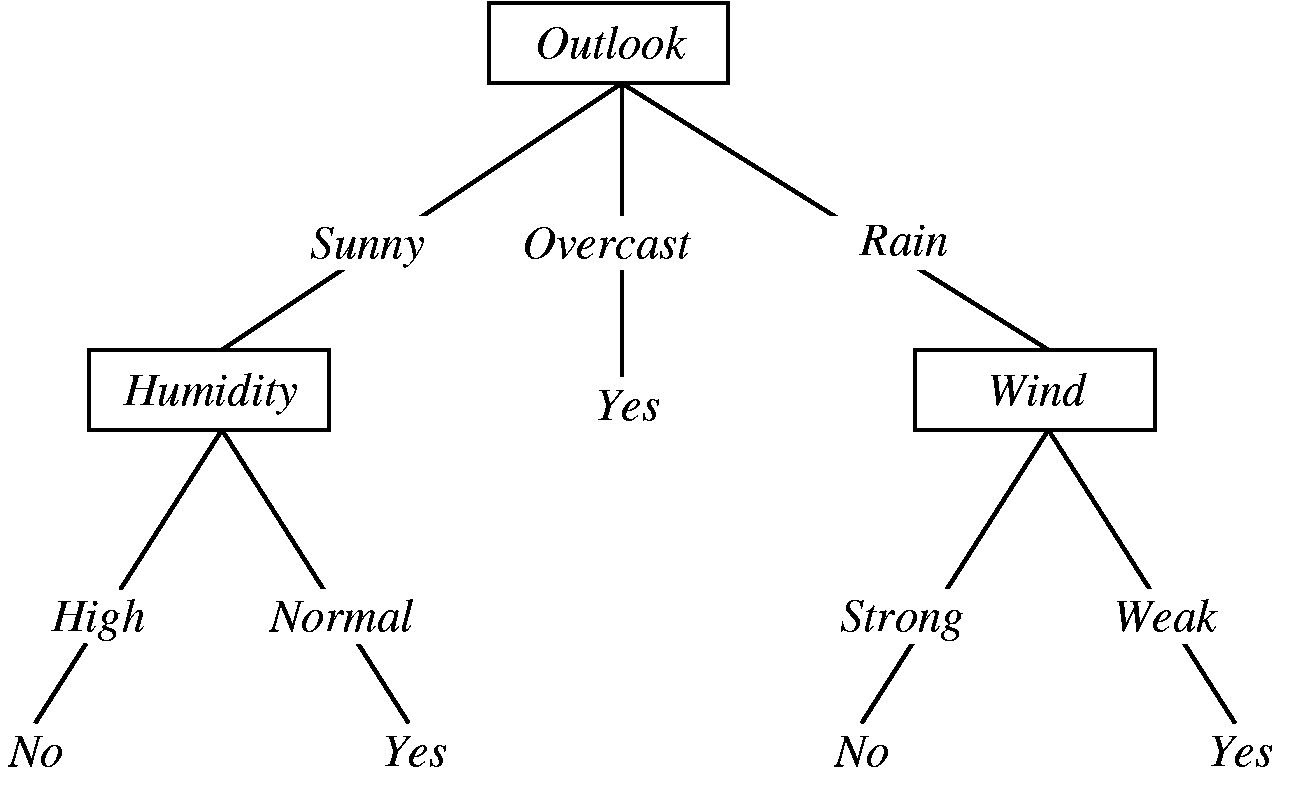
\includegraphics{images/exemple_tree}
\caption{Exemple d'arbre de décision: Permet de décider si nous pouvons aller jouer au tennis ou non.}
\end{figure}

\paragraph{}
Afin de construire l'arbre à partir de l'ensemble d'entraînement, il existe plusieurs algorithmes. Un des plus connus est le \textit{ID3} [\ref{id3}]. Il s'agit d'une méthode de type \textit{greedy} qui va à chaque itération, effectuer un test statistique\footnote{Il vise à vérifier la quantité d'information gagnée pour la classification [\ref{id3}].} afin de savoir quel attribut est le plus discriminant, utilisant cet attribut comme nœud, puis itérer jusqu'à avoir utilisé tous les attributs.


\subsubsection{\textit{Naive Bayes}}
\paragraph{}
À l'instar de la régression logistique [\ref{section régression logistique}], il s'agit d'un classifieur probabiliste. Ce dernier se base sur le théorème de Bayes\footnote{\url{https://brilliant.org/wiki/bayes-theorem/}}:
\begin{center}
$P(Y|X) = \frac{P(X|Y)}{P(X)}P(Y)$
\end{center}
Il est important que les données aient une distribution normale.

À partir de cela, nous obtenons l'équation de \textit{machine learning} suivante [\ref{machine learning automated trading}]:
\begin{center}
$V_{NB} = arg\ max_{v_{j \in V}} P(v_j) \prod\limits_i P(a_i | v_j)$
\end{center}
Où $V_{NB}$ est la classe obtenue, $P(v_j)$ la probabilité à \textit{priori} donc sans informations et $\prod\limits_i P(a_i | v_j)$ la probabilité de vraisemblance.
Il convient donc de trouver la classe qui maximise ce calcule.

\paragraph{}
La \textit{ROC\footnote{Receiver Operating Characteristic} Curve analysis} permet d'améliorer le classifieur. En effet cette dernière peut détecter les \textit{true positive rate} par rapport aux \textit{false positive rate} pour différents seuils de classification de l'algorithme \textit{Naive Bayes} [\ref{machine learning automated trading}]. À partir de cela on peut déterminer le meilleur seuil de sortie et donc perfectionner notre algorithme.
De plus cette courbe peut aider à comparer des classifieurs entre eux en comparant la surface sous la courbe [\ref{machine learning automated trading}].

La méthode utilisée est la suivante [\ref{machine learning automated trading}]: il faut faire s'intersecter la pente $S$ avec la courbe \textit{ROC} et ainsi obtenir une valeur optimale pour le seuil.
Cette pente $S$ est définie comme suit [\ref{machine learning automated trading}]:
\begin{center}
$S = \frac{Cost(P|N) - Cost(N|N)}{Cost(N|P) - Cost(P|P)} \cdot \frac{N}{P}$
\end{center}
Sachant que $Cost(P|N)$ est le coût pour avoir mal classé une classe négative comme positive. $P$ est la somme des vrais positifs et des faux négatifs. $N$,quant à lui, vaut la somme des vrais négatifs ainsi que des faux positifs.

Voici une illustration\footnote{Source: \url{http://www.prolekare.cz/dbpic/jp_5403_f_20-x1000_1600}}:
\begin{figure}[h!]
\centering
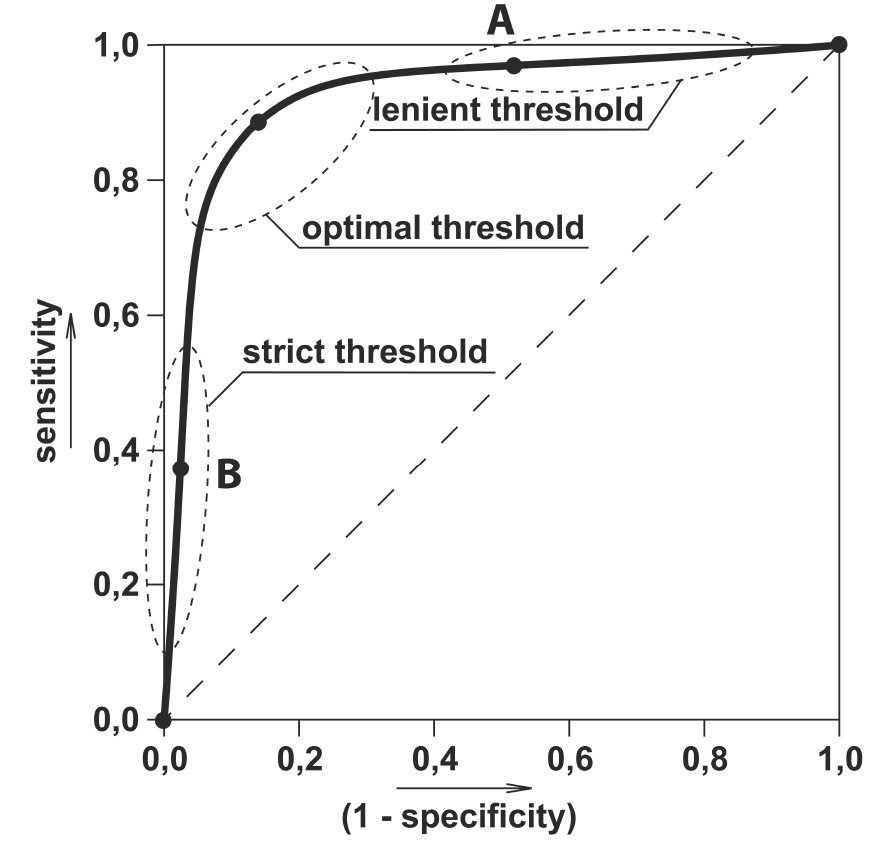
\includegraphics[scale=0.25]{images/roc_curve}
\caption{Exemple de \textit{ROC curve}: L'axe des $x$ correspond au taux de faux positifs et l'axe des $y$ au taux de vrais positifs. On veut donc trendre vers $y = 1$ et $x = 0$. Lors de l'optimisation par la pente $S$, le but sera d'obtenir une intersection avec la \textit{ROC curve} dans la zone \textit{optimal threshold} afin d'avoir le meilleur seuil possible.}
\end{figure}


\subsubsection{\textit{SVM}}
\paragraph{}
Le but de l'algorithme \textit{SVM}\footnote{\textit{Support Vector Machine}} est de séparée les données grâce à un hyper-plan. Cela permet de différencier les classes des observations suivant qu'ils se trouvent d'un côté ou l'autre du plan séparant. Ce plan n'est pas unique\footnote{Source: \url{https://computersciencesource.files.wordpress.com/2010/01/svmafter.png}}: 
\begin{figure}[h!]
\centering
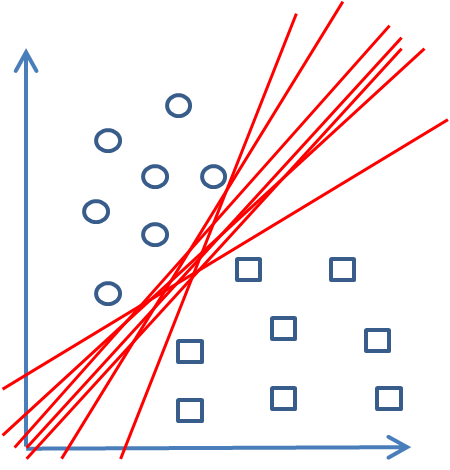
\includegraphics{images/svm_exemple}
\caption{Exemple d'hyper-plans séparant les données. Si nous voulons classifier un nouvel élément, il suffit de calculer s'il se trouve à gauche ou à droite de l'hyper-plan. Dans le premier cas, il s'agira, pour notre algorithme, d'un rond et dans l'autre d'un carré}
\end{figure}

\paragraph{}
Notre fonction est:
\begin{center}
$f(x) = (w \cdot x) + b$
\end{center}
Le but est de maximiser la distance entre les points les plus proches de l'hyper-plan, tout en pénalisant les points mal classés. Il n'est pas toujours possible de séparer les données de dimensions $n$, il conviendra donc d'augmenter la dimension afin d'obtenir une dimension $m > n$. La fonction $\phi(x)$ est utilisée dans ce but. Un exemple de fonction est:
\begin{center}
$\phi: R^2 \rightarrow R^3 (x, y) \rightarrow (x, y, z):= (x^2, \sqrt{2}x y, y^2)$
\end{center}

Il est possible d'imager cette opération comme cela\footnote{\url{https://www.dtreg.com/uploaded/pageimg/SvmDimensionMap.jpg}}:
\begin{figure}[H]
\centering
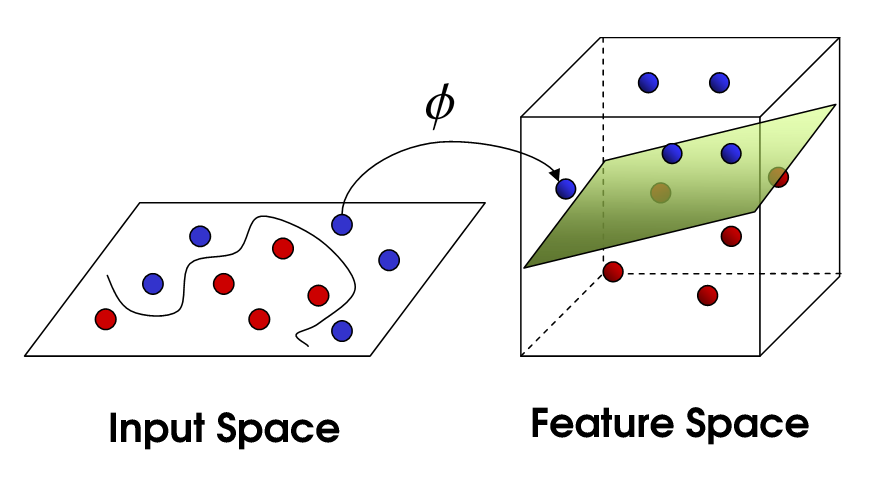
\includegraphics[scale=0.3]{images/svm_exemple_phi}
\caption{Exemple d'utilisation de la fonction $\phi$ pour passer d'un espace $R^2$ à $R^3$ afin de faciliter la séparation.}
\end{figure}


En terme d'équation, nous voulons minimiser w,$||w||^2$ dans l'équation de l'hyper-plan: $(w \cdot x) + b$. Ce qui donne:
\begin{center}
$y_i (w \cdot x_i + b) \ge 1$ si $y \in \{-1, +1\}$ [\ref{svm equation}]
\end{center}
Si malgré l'augmentation de la dimension, les données ne sont pas séparables, il faut tenter de minimiser le nombre d'éléments mal placés. Pour ce faire:
\begin{center}
$y_i (w \cdot x_i + b) \ge 1 - \xi_i$ avec $\xi_i > 0$ [\ref{svm equation}]
\end{center}
Afin de diminuer l'erreur et optimiser au mieux notre classifieur.


\subsubsection{Réseaux de neurones}
\paragraph{}
Tout comme les algorithmes génétiques qui s'inspirent de la sélection naturelle dans un but d'optimisation, les réseaux de neurones se basent sur un modèle formels de neurones\footnote{Neurones formels: \url{http://www.peoi.org/Courses/Coursesfr/neural/neural3.html}} afin de copier la capacité d'apprentissage des êtres vivants.

Il s'agit d'opérer à partir de données en entrée, des \textit{inputs}, une ou plusieurs multiplications matricielles en utilisant des vecteurs de poids, des \textit{weigth}. L'optimisation s'applique sur les \textit{weights}, afin de maximiser la classification.

Un réseau de neurones peut avoir plusieurs couches, \textit{layers}. Dans ce cas, la première couche est appelée \textit{input layer}, la dernière \textit{output layer} et toutes celles entre ces deux sont les \textit{hidden layers}. De plus les neurones peuvent être pleinement connectés avec ceux de la couche suivante, \textit{feed-forward}; ce qui signifie que les neurones de la couche $n-1$ influencent ceux de la couche $n$. À l'opposé, il est possible que ceux en $n$ pèsent sur les neurones de $n-1$, ce phénomène est appelé \textit{feedback networks}.

\begin{figure}[H]
\centering
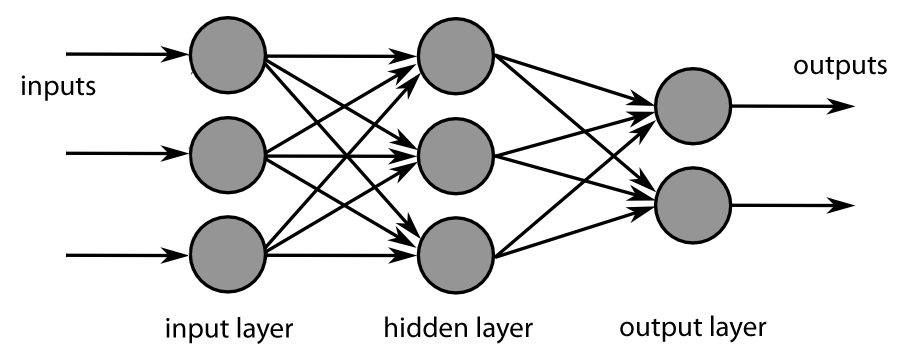
\includegraphics[scale=0.4]{images/neural_net_feedforward}
\caption[]{Exemple de réseau de neurones avec plusieurs couches. Illustre également le \textit{feed-forward}: l'\textit{ouput} de l'\textit{input layer} est propagé dans chaque neurones de l'\textit{hidden layer}. Même chose pour les deux dernières couches.\footnotemark}
\end{figure}

\footnotetext{Source: \url{http://web.utk.edu/~wfeng1/spark/_images/fnn.png}}

\begin{figure}[H]
\centering
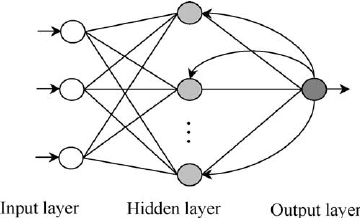
\includegraphics{images/neural_net_feedback}
\caption[]{Exemple de réseau de neurones avec plusieurs couches. Dans ce cas là, les couches sont \textit{feed-forward} mais de plus, le \textit{feedback} est utilisé afin d'influencer les couches précédant l'\textit{output layer}.\footnotemark}
\end{figure}

\footnotetext{Source: \url{https://www.researchgate.net/profile/Yen-Ming_Chiang/publication/222562767/figure/fig2/AS:305112384851969@1449755869325/Fig-2-The-architecture-of-a-recurrent-neural-network.png}}

\paragraph{}
Concernant la valeur de sortie, elle peut être simple. Comme le résultat d'un classification binaire, donc $0$ ou $1$ en sortie. Mais elle peut également être multiple. Il est donc possible d'avoir un résultat étant un vecteur, comme par exemple un point précis dans un espace $R^2$.

Afin de borner les valeurs en sortie, la plupart des réseaux utilisent une fonction. Nous pouvons citer :
\begin{itemize}
\item La fonction sigmoïde : $S(t) = \frac{1}{1 + e^{-t}}$.
\item La fonction tangente hyperbolique : $f(x) = tanh(x)$.
\end{itemize}

Bien souvent, l'utilisation d'un réseau de neurones à une couche est suffisante. Cela est valable pour les fonctions continues, dans le cas de fonctions discontinues, il est intéressant de passer à un réseau disposant de plusieurs couches. Attention toutefois, si le nombre de neurones est trop important, l'algorithme va avoir tendance à sur-apprendre, et à l'inverse, à sous-apprendre si le nombre est trop faible. Il est donc important de bien doser cette quantité afin d'éviter ces problèmes.

\paragraph{}
L'article qui se trouve au coeur du projet [\ref{fx trading}] propose un algorithme basé sur les réseaux de neurones. Il s'agit de trois couches qui doivent chacune une série de paramètres. La première va maximiser la première série de paramètres suivant certain critères. Une fois ces paramètres changés, ils deviennent des constantes pour les deux prochaines couches. La deuxième va améliorer les paramètres qui lui sont attachés en gardant comme les valeurs des paramètres de la première couche constant. Le même principe est répété pour la troisième couche.

Ce n'est donc pas un réseau à multiples couches, dans le sens où, une série de paramètres n'est optimisée que par une couche et non plusieurs. On peut visualiser cela comme trois réseaux qui chaînent leurs résultats.

\subsubsection{Descente du gradient}
\paragraph{}
L'algorithme de descente du gradient fonctionne sur des fonctions réelles différentiables sur un espace tel quel $\mathbb{R}^n$. Il est itératif est fonctionne donc en améliorant l'itération précédente, jusqu'à atteindre une condition d'arrêt.

Avant d'en expliquer la teneur mathématique, voici un exemple de l'algorithme dans $\mathbb{R}^2$ :

\begin{figure}[H]
\centering
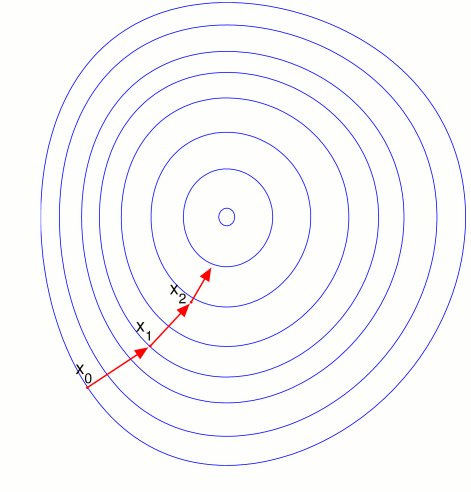
\includegraphics[scale=0.40]{images/descente_gradient_exemple}
\caption[]{Exemple de l'algorithme de descente du gradient en deux dimensions. À chaque itération, il faut prendre la direction opposée au gradient\footnotemark, cela permet d'arriver à un nouveau point. En itérant, on se rapproche de l'maximum. }
\end{figure}

\footnotetext{Dans cet exemple, il est possible de dire, qu'il faut prendre la normal de la courbe de niveau.}

\paragraph{}
Afin de comprendre, les divers algorithmes, il est important d'avoir les connaissances mathématiques sur ce sujet. L'algorithme se définit comme suit :

\paragraph{}
\footnote{Inspiré de [\ref{wikipedia descente du gradient}]}Soit un point initial $x_0 \in \mathbb{R}$. Soit $\epsilon > 0$ un seuil de tolérance. L'algorithme définit une suite d'itération $x_1,x_2,.. \in \mathbb{R}^n$, jusqu'à ce qu'un test d'arrêt soit satisfait. Pour passer de $x_i$ à $x_{i+1}$, il faut :
\begin{itemize}
\item Calculer $\bigtriangledown f(x_k)$
\item Si $||\bigtriangledown f(x_k) \le \epsilon$ alors arrêt.
\item Sinon il faut calculer $\alpha_k$ par recherche linéaire sur $f$ en $x_k$. Cette recherche se fait dans la direction opposée au gradient, soit $-\bigtriangledown f(x_k)$. Une fois $\alpha_k$ calculé, il faut mettre à jour le point itéré : $$x_{k+1} = x_k - \alpha_k \bigtriangledown f(x_k)$$
\end{itemize}

\paragraph{}
La preuve que la recherche dans la direction opposée au gradient induit une décroissance est la suivante.
Si la dérivée est non nulle au point $x$\footnote{i.e: Si nous ne sommes pas déjà sur un maximum}, $f'(x) \ne 0$. Soit
$$d = - \bigtriangledown f(x)$$
Puisque :
$$f'(x) \cdot d = \bigtriangledown f(x) \cdot -\bigtriangledown f(x) = - ||\bigtriangledown f(x) ||^2 < 0$$

Nous avons un strictement plus petit car la dérivée est non nulle par hypothèse. Cela implique que :
$$f(x -\alpha \bigtriangledown f(x)) < f(x)\text{,\ } \forall \alpha > 0$$

Nous avons donc que pour chaque itération, la valeur obtenue va décroître jusqu'à attendre un maximum ou le seuil $\epsilon$.

\paragraph{}
La descente du gradient d'un point de vue mathématique peut également être utilisée conjointement à un réseau de neurones. En effet dans cet article [\ref{fx trading}], les poids $w$ de la première couche, sont optimisés suivant cette formule :
$$w_{i,t} = w_{i-1,t} + \rho \bigtriangleup w_{i,t}$$

Où $t$ correspond au temps, $i-1$ à l'itération courante et $\rho$ le taux d'apprentissage.
De part la convergence de $w_i$ vers son optimale, cela permet, une fois cette valeur obtenue, de l'injecter comme étant les poids d'un réseau de neurones.

\paragraph{}
Il existe deux types d'algorithme de descente du gradient :
\begin{itemize}
\item Le \textit{Batch Algorithm} a pour but de minimiser la fonction de coût qui aura été définie au préalable. Ce dernier peut prendre énormément de temps sur des gros jeux de données de par son côté itératif.
\item Le \textit{Online Algorithm} va prendre les exemples un à un. L'optimisation ne va se faire que pour cet unique exemple puis va recommencer sur une autre donnée. Cette manière de procéder s'applique aisément sur les gros volumes de données.
\end{itemize}

Tiré cet article [\ref{descente du gradient stochastique}], voici des équations pouvant être minimisée dans le cadre d'un programme de \textit{machine learning}.
Soit $(x_i,y_i)\text{,\ } i=1..N$, un ensemble de données. Notre fonction de coût est $l(y,y')$. Cela représente le coût de prédire $y'$ quand la réponse est $y$. Moyennons cela sur tous les exemples :
$$E_N(f) = \frac{1}{N} \sum_{i=1}^{n}l(f_w(x_i),y_i)$$
Où $f_w$ est une fonction pondérée par un vecteur de poids $w$ que l'on cherche à optimiser.
Pour optimiser les poids, nous allons utiliser la descente du gradient :
$$w_{k+1} = w_k - \alpha_k \bigtriangledown f_{w_k}(x) \rightarrow w_{k+1} = w_k -\alpha_k \sum_{i=1}^n \bigtriangledown Q ((x_i,y_i), w_k)$$

Où $Q(x,y) = l(f_w(x),y)$.

\paragraph{}
Comme mentionné plus haut, la technique de \textit{Batch Algorithm} devient lente lorsque la taille du jeu de données augmente. Pour pallier à ce problème, il existe une technique : \textit{stochastic gradient descent}. C'est une méthode d'approximation statistique de la descente du gradient.

Il convient de ne prendre qu'un seul couple au lieu de l'ensemble complet d'entraînement. La somme disparaît donc dans l'équation à minimiser :
$$w_{k+1} = w_k -\alpha_k \bigtriangledown Q ((x_i,y_i), w_k)$$
C'est donc une technique de \textit{Online Algorithm}. De part le fait qu'il n'a pas besoin de se souvenir des exemples précédant, l'algorithme peut traiter des données à la volée.

Il est possible pour pénaliser la complexité de $w$ de rajouter un élément. Cela d'essayer de borner les valeurs des poids:
$$w_{k+1} = w_k -\alpha_k \bigtriangledown Q ((x_i,y_i), w_k) + \sigma P(w_k)$$

Où $\sigma > 0$ est un hyper-paramètre et $P$ peut valoir :
\begin{itemize}
\item \textbf{L1 norm} = $P(w) := \sum\limits_{i=1}^n |w_i|$
\item \textbf{L2 norm} = $P(w) := \frac{1}{2}\sum\limits_{i=1}^n w_i^2$
\item \textbf{Elastic Net} = $P(w) := \rho \frac{1}{2}\sum\limits_{i=1}^n w_i^2 + (1 - \rho) \sum\limits_{i=1}^n |w_i|$
\end{itemize}


\subsection{\textit{Machine Learning} dans le cadre de la finance}
\paragraph{}
Avant de parler des performances des algorithmes mentionnés, il convient de préciser qu'ils proviennent de plusieurs articles et recherches différents. Ils ont donc été testé avec des paramètres ayant des valeurs disparates ainsi que sur des données distinctes.
Il est donc très compliqué de comparer les résultats des algorithmes et d'affirmer qu'une méthode est meilleure qu'une autre. Ces résultats servent plutôt à illustrer la qualité intrinsèque des procédés. Avec un résultat de 80\%, nous pouvons estimer que la performance est bonne, et l'inverse pour une valeur de 20\%.
\subsection{Conclusion}
\newpage
%%%%%%%%%%%%%%%%%%%%%%%%%%%%%%%%%%%%%%%%%%%%%%%%%%%%%%%%%%%%%%%%%%%%%%%%%%
% début du projet  %%%%%%%%%%%%%%%%%%%%%%%%%%%%%%%%%%%%%%%%%%%%%%%%%%%%%%%
%%%%%%%%%%%%%%%%%%%%%%%%%%%%%%%%%%%%%%%%%%%%%%%%%%%%%%%%%%%%%%%%%%%%%%%%%%
\section{Projet}
\newpage
%%%%%%%%%%%%%%%%%%%%%%%%%%%%%%%%%%%%%%%%%%%%%%%%%%%%%%%%%%%%%%%%%%%%%%%%%%
% début de la bibliographie %%%%%%%%%%%%%%%%%%%%%%%%%%%%%%%%%%%%%%%%%%%%%%
%%%%%%%%%%%%%%%%%%%%%%%%%%%%%%%%%%%%%%%%%%%%%%%%%%%%%%%%%%%%%%%%%%%%%%%%%%
\section{Bibliographie}

\begin{enumerate}
\item "\textit{An automated fx trading system using adaptive reinforcement learning}" de M.A.H Dempster et V. Leemans 2004. \label{fx trading}
\item Financial Times: "\textit{Real investors eclipsed by fast trading}", 2012 \url{https://www.ft.com/content/da5d033c-8e1c-11e1-bf8f-00144feab49a?mhq5j=e1} \label{real investors}
\item "\textit{A Machine Learning Approach to Automated Trading}", 09.05.2016, Ning Lu \label{machine learning automated trading}
\item "\textit{An efficient implementation of the backtesting of trading strategies.}" Ni, Jiarui, et Chegqi Zhang, \textit{Parallel and Distributed Processing and Applications} (2005): 126-131.
\item "\textit{Algorithmic Trading: Winning Strategies and Their Rationale ( Wiley Trading Series)}", John Wiley and Sons, 2013
\item "\textit{Machine Learning}", Mitchell, Tom M. New York, 1997. \label{mitchell}
\item Article Wikipédia sur SVM: \url{https://fr.wikipedia.org/wiki/Machine_\%C3\%A0_vecteurs_de_support} \label{wikipedia svm}
\item "\textit{Online Machine Learning Algorithms For Currency Exchange Prediction}", Eleftherios Soulas et Dennis Shasha de NYU, Courant Department. \label{descente du gradient stochastique}
\item  Article Wikipédia sur Algorithme du gradient: \url{https://fr.wikipedia.org/wiki/Algorithme_du_gradient} \label{wikipedia descente du gradient}
\item "\textit{Descision Tree Learning}", Tom M. Mitchell \label{id3}
\item Article Investopedia sur les Options \url{http://www.investopedia.com/terms/o/option.asp}
\item "\textit{Support Vector Machine (and Statistical Learning Theory) Tutorial}", de Jason Weston, NEC Labs America. \url{http://www.cs.columbia.edu/~kathy/cs4701/documents/jason_svm_tutorial.pdf} \label{svm equation}
\item  "\textit{An Introduction to Neural Networks}" Vincent Cheung et Kevin Cannons: \url{http://www2.econ.iastate.edu/tesfatsi/NeuralNetworks.CheungCannonNotes.pdf}
\item Exemple de réseaux de neurones\url{http://csc.lsu.edu/~jianhua/nn.pdf} p.5
\item \textit{Backtesting} Investopedia \url{http://www.investopedia.com/terms/b/backtesting.asp} \label{backtesting investopedia}
\item Historique des taux de changes: \url{http://www.xe.com/currencycharts/} \label{historique taux de change}
\item Article Wikipedia sur les Accords de Bretten Woods: \url{https://fr.wikipedia.org/wiki/Accords_de_Bretton_Woods} \label{wikipedia bretten woods}
\item Article Étalon-Or à Étalon-Dollar: \url{http://la-chronique-agora.com/etalon-or-etalon-dollar/} \label{étalon-or à étalon-dollar}
\item \textit{CHAPITRE 1: LE MARCHE DES CHANGES Monnaie et Finance Internationales} de David Guerreiro, Université Paris 8, \url{https://economix.fr/docs/1045/chap_1_2015-16.pdf} \label{marche des changes}
\item Site \textit{FOREX} français: \url{http://www.forex.fr/newslist/8696-la-regle-des-trois-unites-du-marche-des-changes} \label{site fr forex}
\item Investopedia Bid-Ask: \url{http://www.investopedia.com/terms/b/bid-and-asked.asp} \label{investopedia bid ask}
\item Wikipédia Broker: \url{https://en.wikipedia.org/wiki/Broker} \label{wikipedia broker}
\item Wikipédia Régression Statistique: \url{https://fr.wikipedia.org/wiki/R\%C3\%A9gression_(statistiques)} \label{wikipedia régression}
\end{enumerate}


\end{document}